\documentclass[12pt]{report}

\usepackage{amsmath}
\usepackage{textcomp}
\usepackage{gensymb}
\usepackage{bookmark} % added to see what happens
\usepackage{framed} % added to see what happens. These two packages were in response to some errors that latex kept throwing me
% when compiling the test templates
% this is to see if I can sneak in using cochineal


% use of color
\usepackage{xcolor}


\providecommand{\keywords}[1]{\textbf{\textit{Keywords---}}#1}


\providecommand{\titlediss}{Testing the Effect of something on something
else}
% name in caps
\providecommand{\writerUpper}{JOSH ALLEN}
% name normal
\providecommand{\writerLower}{Josh Allen}
\providecommand{\chair}{Ellen Ripley}

\providecommand{\committeeOne}{Bruce Banner}
\providecommand{\committeeTwo}{Indiana Jones}
%%% if you have more than one committee member just add that right here
\providecommand{\gradMonth}{May}
\providecommand{\gradYear}{2022}

\renewenvironment{abstract}{
\begin{center}
{ABSTRACT \vspace{0.2in}}
\end{center}
}{}

\providecommand{\keywordOne}{keyword1}
\providecommand{\keywordTwo}{keyword2}

\providecommand{\Chapter}[2]{\chapter[#1]{#1 \\ \begin{flushleft} \footnotesize \textit{#2} \normalsize \end{flushleft}}}

% renames 'Contents' to 'Table of Contents'
\renewcommand{\contentsname}{Table of Contents}



% allows use of citet and citep

% make sure you are citing everything listed!!! comment out to prevent latex getting mad about unlabelled equations and figures
%\usepackage{refcheck}
% removes commas after et al. in \citep to match AAS and MNRAS formatting
%\setcitestyle{aysep={}}


\usepackage{csquotes}
\usepackage[natbib,authordate,backend=biber,sorting=nyt]{biblatex-chicago}
\addbibresource{ref.bib}


\usepackage{color}
\usepackage{fancyvrb}
\newcommand{\VerbBar}{|}
\newcommand{\VERB}{\Verb[commandchars=\\\{\}]}
\DefineVerbatimEnvironment{Highlighting}{Verbatim}{commandchars=\\\{\}}
% Add ',fontsize=\small' for more characters per line
\usepackage{framed}
\definecolor{shadecolor}{RGB}{241,243,245}
\newenvironment{Shaded}{\begin{snugshade}}{\end{snugshade}}
\newcommand{\AlertTok}[1]{\textcolor[rgb]{0.68,0.00,0.00}{#1}}
\newcommand{\AnnotationTok}[1]{\textcolor[rgb]{0.37,0.37,0.37}{#1}}
\newcommand{\AttributeTok}[1]{\textcolor[rgb]{0.40,0.45,0.13}{#1}}
\newcommand{\BaseNTok}[1]{\textcolor[rgb]{0.68,0.00,0.00}{#1}}
\newcommand{\BuiltInTok}[1]{\textcolor[rgb]{0.00,0.23,0.31}{#1}}
\newcommand{\CharTok}[1]{\textcolor[rgb]{0.13,0.47,0.30}{#1}}
\newcommand{\CommentTok}[1]{\textcolor[rgb]{0.37,0.37,0.37}{#1}}
\newcommand{\CommentVarTok}[1]{\textcolor[rgb]{0.37,0.37,0.37}{\textit{#1}}}
\newcommand{\ConstantTok}[1]{\textcolor[rgb]{0.56,0.35,0.01}{#1}}
\newcommand{\ControlFlowTok}[1]{\textcolor[rgb]{0.00,0.23,0.31}{#1}}
\newcommand{\DataTypeTok}[1]{\textcolor[rgb]{0.68,0.00,0.00}{#1}}
\newcommand{\DecValTok}[1]{\textcolor[rgb]{0.68,0.00,0.00}{#1}}
\newcommand{\DocumentationTok}[1]{\textcolor[rgb]{0.37,0.37,0.37}{\textit{#1}}}
\newcommand{\ErrorTok}[1]{\textcolor[rgb]{0.68,0.00,0.00}{#1}}
\newcommand{\ExtensionTok}[1]{\textcolor[rgb]{0.00,0.23,0.31}{#1}}
\newcommand{\FloatTok}[1]{\textcolor[rgb]{0.68,0.00,0.00}{#1}}
\newcommand{\FunctionTok}[1]{\textcolor[rgb]{0.28,0.35,0.67}{#1}}
\newcommand{\ImportTok}[1]{\textcolor[rgb]{0.00,0.46,0.62}{#1}}
\newcommand{\InformationTok}[1]{\textcolor[rgb]{0.37,0.37,0.37}{#1}}
\newcommand{\KeywordTok}[1]{\textcolor[rgb]{0.00,0.23,0.31}{#1}}
\newcommand{\NormalTok}[1]{\textcolor[rgb]{0.00,0.23,0.31}{#1}}
\newcommand{\OperatorTok}[1]{\textcolor[rgb]{0.37,0.37,0.37}{#1}}
\newcommand{\OtherTok}[1]{\textcolor[rgb]{0.00,0.23,0.31}{#1}}
\newcommand{\PreprocessorTok}[1]{\textcolor[rgb]{0.68,0.00,0.00}{#1}}
\newcommand{\RegionMarkerTok}[1]{\textcolor[rgb]{0.00,0.23,0.31}{#1}}
\newcommand{\SpecialCharTok}[1]{\textcolor[rgb]{0.37,0.37,0.37}{#1}}
\newcommand{\SpecialStringTok}[1]{\textcolor[rgb]{0.13,0.47,0.30}{#1}}
\newcommand{\StringTok}[1]{\textcolor[rgb]{0.13,0.47,0.30}{#1}}
\newcommand{\VariableTok}[1]{\textcolor[rgb]{0.07,0.07,0.07}{#1}}
\newcommand{\VerbatimStringTok}[1]{\textcolor[rgb]{0.13,0.47,0.30}{#1}}
\newcommand{\WarningTok}[1]{\textcolor[rgb]{0.37,0.37,0.37}{\textit{#1}}}
% for figures
\usepackage{graphicx}
\usepackage{epstopdf}
\usepackage{longtable}

% appendices for chapters
\usepackage{appendix}

% allows rotations
\usepackage{pdflscape}

% allows for use of \cmidrule
\usepackage{booktabs}

% for caption stuff
\usepackage{caption}

% line spacing, whatever
\usepackage{microtype}

% float control
\usepackage{float}

% sets 1 inch margins
\usepackage[margin=1in]{geometry}

% binding offset
% ONLY USE ONCE DOCUMENT IS READY FOR PRINTING!
% CHANGES PAGE LAYOUT!
%\usepackage[margin=1in, twoside, bindingoffset=0.5in]{geometry}

% sets spacing to double spaced
\usepackage{setspace}
\doublespacing

% makes section (etc.) titles 12 pt font
\usepackage{titlesec}
\titleformat*{\section}{\fontsize{12}{15}\bfseries}
\titleformat*{\subsection}{\fontsize{12}{15}\bfseries}
\titleformat*{\subsubsection}{\fontsize{12}{15}\bfseries}

% sets depth of subsections, match this with how deep you go above
\setcounter{secnumdepth}{3}

% makes chapter titles 12 pt font
\titleformat{\chapter}[display]
{\normalfont \bfseries\centering}
{\chaptertitlename\ \thechapter}{12pt}
{\normalfont \bfseries\centering}

% hyper ref without coloring the links
\usepackage{hyperref}
\hypersetup{
    colorlinks,
    citecolor=black,
    filecolor=black,
    linkcolor=black,
    pdfkeywords = {},
    urlcolor=black,
    linktoc=all}

% prevent widows and orphans, or at least makes LaTeX try really hard to do so
\usepackage[all,defaultlines=2]{nowidow}

% lets just hard code this for now
\usepackage{fancyhdr}
\pagestyle{fancy}
\fancyhf{}
\renewcommand{\headrulewidth}{0pt}
\fancyhead[R]{\thepage}


\begin{document}

\thispagestyle{empty}

\begin{center}
\parbox[]{\textwidth}{\setstretch{2}\centering\titlediss}
\end{center}
\vspace{0.4in}
\centerline{by}
\vspace*{0.5in}
\centerline{JOSH ALLEN}
\vspace*{0.5in}
\centerline{Under the Direction of Ellen Ripley, PhD}
\vspace{1.0in}



\centerline{A Dissertation Submitted in Partial Fulfillment of the Requirements of }
\centerline{Doctor of Philosophy}
\centerline{in the College of Arts and Sciences}
\centerline{Georgia State University}
\centerline{2022}
\newpage

\newpage

\thispagestyle{empty}

\begin{abstract}




\end{abstract}
\begin{singlespace}
  \vspace{0.5in}
  \noindent Index words: 
  \hspace{0.2in}
  \parbox[t]{4.5in}{These, Are, Tests}
\end{singlespace}

\newpage

\thispagestyle{empty}

\vspace*{0.7\textheight}
\begin{center}
  \parbox[]{\textwidth}{\setstretch{1}
    \begin{center}
      Copyright by \\
      Josh Allen \\
      2022
    \end{center}}
\end{center}

\newpage

% FRONT MATTER

\thispagestyle{empty}



\begin{center}
  \parbox[]{\textwidth}{\setstretch{2}\centering \titlediss}
  \end{center}

  \vspace*{0.5in}
  \centerline{by}
  \vspace*{0.5in}
  \centerline{JOSH ALLEN}
  \vspace*{1in}

  \hspace{0.33\textwidth}
  \begin{minipage}[t]{0.33\textwidth}
  Committee Chair:\\
  Committee: \\
  \end{minipage}%
  \begin{minipage}[t]{0.33\textwidth}
  \begin{flushright}
  Ellen Ripley \\
  Bruce Banner \\
  Indiana Jones \\
  \end{flushright}
  \end{minipage}%
  \vspace{1cm}

  \parbox[b]{\textwidth}{\setstretch{2}
  Electronic Version Approved:\\\\\\
  Office of Graduate Studies\\
  College of Arts and Sciences\\
  Georgia State University\\
  May 2022
  }



\thispagestyle{empty}
\setlength{\abovedisplayskip}{-5pt}
\setlength{\abovedisplayshortskip}{-5pt}
% this is where you should break it up



\bookmarksetup{startatroot}

\hypertarget{dedication}{%
\chapter*{Dedication}\label{dedication}}
\addcontentsline{toc}{chapter}{Dedication}

\markboth{Dedication}{Dedication}

this is dedicated to the haters

\setcounter{page}{4}
\pagenumbering{roman}
\pagestyle{fancy}

\bookmarksetup{startatroot}

\hypertarget{acknowledgements}{%
\chapter*{Acknowledgements}\label{acknowledgements}}
\addcontentsline{toc}{chapter}{Acknowledgements}

\markboth{Acknowledgements}{Acknowledgements}

I would like to thank my pet goldfish for \ldots{}

\pagenumbering{roman}
\setcounter{page}{4}

\tableofcontents
\newpage

\phantomsection
\addcontentsline{toc}{chapter}{\texorpdfstring{\listtablename \dotfill}{\listtablename}}
\listoftables
\newpage

\phantomsection
\addcontentsline{toc}{chapter}{\texorpdfstring{\listtablename \dotfill}{\listtablename}}
\listoffigures
\newpage

\bookmarksetup{startatroot}

\hypertarget{abreviations}{%
\chapter*{Abreviations}\label{abreviations}}
\addcontentsline{toc}{chapter}{Abreviations}

\markboth{Abreviations}{Abreviations}

abc = the abcs

\cleardoublepage
\pagenumbering{arabic}
\markright{\thepage}
\newpage
\pagenumbering{arabic}

\bookmarksetup{startatroot}

\hypertarget{introduction}{%
\chapter{Introduction}\label{introduction}}

Do you see any Teletubbies in here? Do you see a slender plastic tag
clipped to my shirt with my name printed on it? Do you see a little
Asian child with a blank expression on his face sitting outside on a
mechanical helicopter that shakes when you put quarters in it? No? Well,
that's what you see at a toy store. And you must think you're in a toy
store, because you're here shopping for an infant named Jeb.

\hypertarget{data}{%
\section{Data}\label{data}}

Included in this template is a file called \texttt{sales.csv}. This
contains quarterly data on Sales and Advertising budget for a small
company over the period 1981--2005. It also contains the GDP (gross
domestic product) over the same period. All series have been adjusted
for inflation. We can load in this data set using the following code:

\begin{Shaded}
\begin{Highlighting}[]
\FunctionTok{library}\NormalTok{(palmerpenguins)}

\NormalTok{penguins }\SpecialCharTok{|\textgreater{}}
\FunctionTok{select}\NormalTok{(species, island) }\SpecialCharTok{|\textgreater{}}
\FunctionTok{head}\NormalTok{(}\DecValTok{2}\NormalTok{) }\SpecialCharTok{|\textgreater{}}
\NormalTok{knitr}\SpecialCharTok{::}\FunctionTok{kable}\NormalTok{(}\AttributeTok{format =} \StringTok{"latex"}\NormalTok{)}
\end{Highlighting}
\end{Shaded}

\begin{table}
\caption{this is the data}\tabularnewline

\centering
\begin{tabular}{l|l}
\hline
species & island\\
\hline
Adelie & Torgersen\\
\hline
Adelie & Torgersen\\
\hline
\end{tabular}
\end{table}

Any data you use in your thesis can go into the \texttt{data} directory.
The data should be in exactly the format you obtained it. Do no editing
or manipulation of the data prior to including it in the \texttt{data}
directory. Any data munging should be scripted and form part of your
thesis files (possibly hidden in the output).

\hypertarget{figures}{%
\section{Figures`}\label{figures}}

Figure~\ref{fig-pengs} shows time plots of the data we just loaded.
Notice how figure captions and references work. Chunk names can be used
as figure labels with \texttt{fig-} prefixed. Never manually type figure
numbers, as they can change when you add or delete figures. This way,
the figure numbering is always correct.

\begin{verbatim}
`stat_bin()` using `bins = 30`. Pick better value with `binwidth`.
\end{verbatim}

\begin{verbatim}
Warning: Removed 2 rows containing non-finite values (`stat_bin()`).
\end{verbatim}

\begin{figure}

{\centering 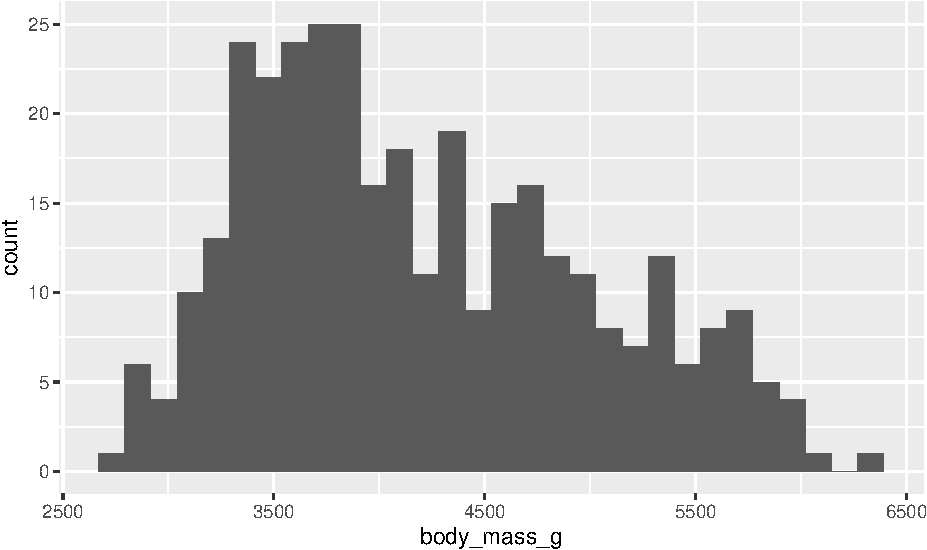
\includegraphics{01-chap1_files/figure-pdf/fig-pengs-1.pdf}

}

\caption{\label{fig-pengs}Quarterly sales, advertising and GDP data.}

\end{figure}

\bookmarksetup{startatroot}

\hypertarget{literature-review}{%
\chapter{Literature Review}\label{literature-review}}

This chapter contains a summary of the context in which your research is
set.

Imagine you are writing for your fellow PhD students. Topics that are
well-known to them do not have to be included here. But things that they
may not know about should be included.

Resist the temptation to discuss everything you've read in the last few
years. And you are not writing a textbook either. This chapter is meant
to provide the background necessary to understand the material in
subsequent chapters. Stick to that.

You will need to organize the literature review around themes, and
within each theme provide a story explaining the development of ideas to
date. In each theme, you should get to the point where your ideas will
fit in. But leave your ideas to later chapters. This way it is clear
what has been done beforehand, and what new contributions you are making
to the research field.

All citations should be done using markdown notation as shown below.
This way, your bibliography will be compiled automatically and
correctly.

\hypertarget{various-lit}{%
\section{Various lit}\label{various-lit}}

One time \textcite{achenBlindRetrospectionElectoral2002} said something
about sharks and then \textcite{fowlerSharkAttacksInfluence2018} and
thus the great shark debate started

% BACK MATTER
\phantomsection
\addcontentsline{toc}{chapter}{Bibliography}

\newpage



		\printbibliography
		
\end{document}
